\documentclass{standalone}
\usepackage{tikz}

\usetikzlibrary{math}

\begin{document}

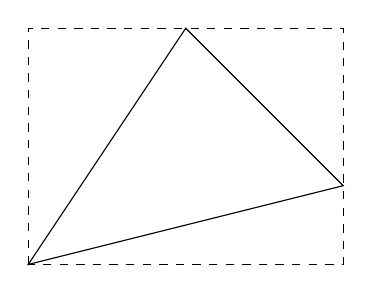
\begin{tikzpicture}
  \tikzmath{
    real \ax,\ay,\bx,\by,\cx,\cz,\Left,\Top,\Right,\Bottom;
    \ax=0;
    \ay=0;
    \bx=4;
    \by=1;
    \cx=2;
    \cy=3;
    \Left=min(\ax,\bx,\cx);
    \Right=max(\ax,\bx,\cx);
    \Top=max(\ay,\by,\cy);
    \Bottom=min(\ay,\by,\cy);
  }
  \coordinate (p1) at (\ax,\ay);
  \coordinate (p2) at (\bx,\by);
  \coordinate (p3) at (\cx,\cy);

  \draw (p1) -- (p2) -- (p3) -- cycle;
  \draw[dashed] (\Left,\Bottom) rectangle (\Right,\Top);
\end{tikzpicture}

\end{document}